\documentclass[]{article}
\usepackage{lmodern}
\usepackage{amssymb,amsmath}
\usepackage{ifxetex,ifluatex}
\usepackage{fixltx2e} % provides \textsubscript
\ifnum 0\ifxetex 1\fi\ifluatex 1\fi=0 % if pdftex
  \usepackage[T1]{fontenc}
  \usepackage[utf8]{inputenc}
\else % if luatex or xelatex
  \ifxetex
    \usepackage{mathspec}
  \else
    \usepackage{fontspec}
  \fi
  \defaultfontfeatures{Ligatures=TeX,Scale=MatchLowercase}
\fi
% use upquote if available, for straight quotes in verbatim environments
\IfFileExists{upquote.sty}{\usepackage{upquote}}{}
% use microtype if available
\IfFileExists{microtype.sty}{%
\usepackage{microtype}
\UseMicrotypeSet[protrusion]{basicmath} % disable protrusion for tt fonts
}{}
\usepackage[margin=1in]{geometry}
\usepackage{hyperref}
\hypersetup{unicode=true,
            pdftitle={Project 1},
            pdfborder={0 0 0},
            breaklinks=true}
\urlstyle{same}  % don't use monospace font for urls
\usepackage{graphicx,grffile}
\makeatletter
\def\maxwidth{\ifdim\Gin@nat@width>\linewidth\linewidth\else\Gin@nat@width\fi}
\def\maxheight{\ifdim\Gin@nat@height>\textheight\textheight\else\Gin@nat@height\fi}
\makeatother
% Scale images if necessary, so that they will not overflow the page
% margins by default, and it is still possible to overwrite the defaults
% using explicit options in \includegraphics[width, height, ...]{}
\setkeys{Gin}{width=\maxwidth,height=\maxheight,keepaspectratio}
\IfFileExists{parskip.sty}{%
\usepackage{parskip}
}{% else
\setlength{\parindent}{0pt}
\setlength{\parskip}{6pt plus 2pt minus 1pt}
}
\setlength{\emergencystretch}{3em}  % prevent overfull lines
\providecommand{\tightlist}{%
  \setlength{\itemsep}{0pt}\setlength{\parskip}{0pt}}
\setcounter{secnumdepth}{0}
% Redefines (sub)paragraphs to behave more like sections
\ifx\paragraph\undefined\else
\let\oldparagraph\paragraph
\renewcommand{\paragraph}[1]{\oldparagraph{#1}\mbox{}}
\fi
\ifx\subparagraph\undefined\else
\let\oldsubparagraph\subparagraph
\renewcommand{\subparagraph}[1]{\oldsubparagraph{#1}\mbox{}}
\fi

%%% Use protect on footnotes to avoid problems with footnotes in titles
\let\rmarkdownfootnote\footnote%
\def\footnote{\protect\rmarkdownfootnote}

%%% Change title format to be more compact
\usepackage{titling}

% Create subtitle command for use in maketitle
\newcommand{\subtitle}[1]{
  \posttitle{
    \begin{center}\large#1\end{center}
    }
}

\setlength{\droptitle}{-2em}
  \title{Project 1}
  \pretitle{\vspace{\droptitle}\centering\huge}
  \posttitle{\par}
  \author{}
  \preauthor{}\postauthor{}
  \date{}
  \predate{}\postdate{}


\begin{document}
\maketitle

\section{Introduction}\label{introduction}

This is Project 1 for STAT 557 2018 Spring by Meridith Bartley and Fei.
The aim of this project is to practice linear classification methods and
QDA and study basic techniques of dimension reduction.In this project we
(1) apply LDA, QDA, and multinomial logistic regression to soil sample
data in order to calssify into separate soil group (Orders).

\section{Description of Data}\label{description-of-data}

This is Fei's research data. It's about soil sample data over the US
downloaded from NRCS, including the physical and chemical properties of
soil samples (sand, silt, clay, oganic carbon, bulk density, CEC soil,
CEC clay, base satuaration, and pH) and the corresponding soil
classification group (soil order).

Boxplots for each physical and chemical property used as explanitory
variables in the subsequent classification models are included below.
This EDA allows for early indication of which variables may possibly be
ommitted during dimention reduction. That is, what properties do not
differ significantly between soil Orders.

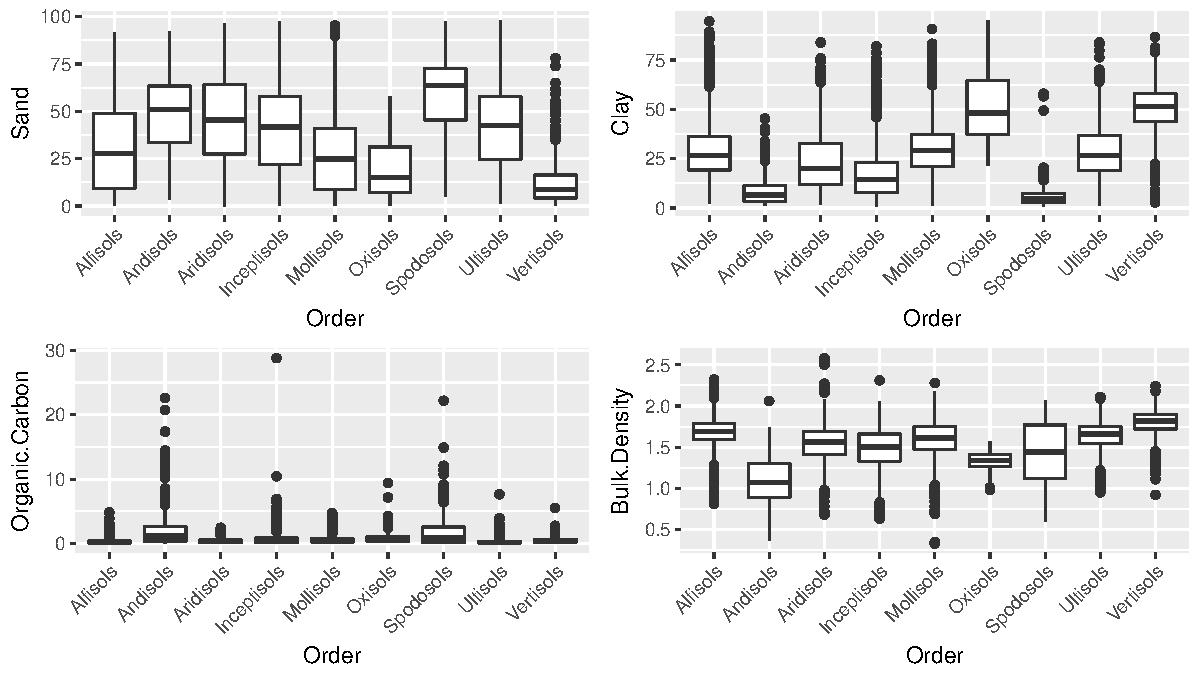
\includegraphics{Project1_files/figure-latex/EDA - Mer-1.pdf}
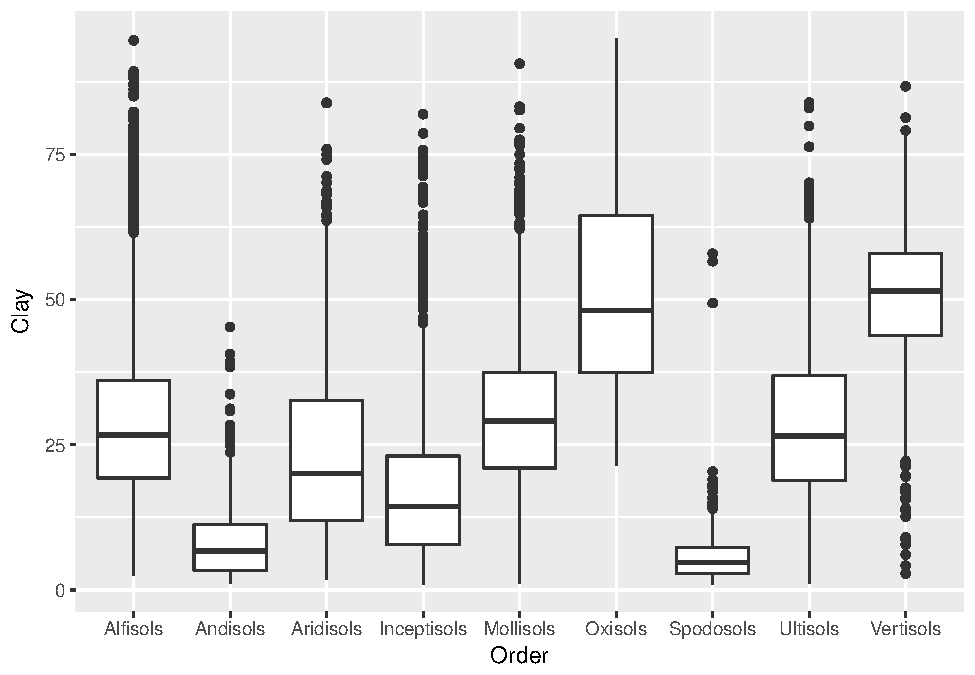
\includegraphics{Project1_files/figure-latex/EDA - Mer-2.pdf}
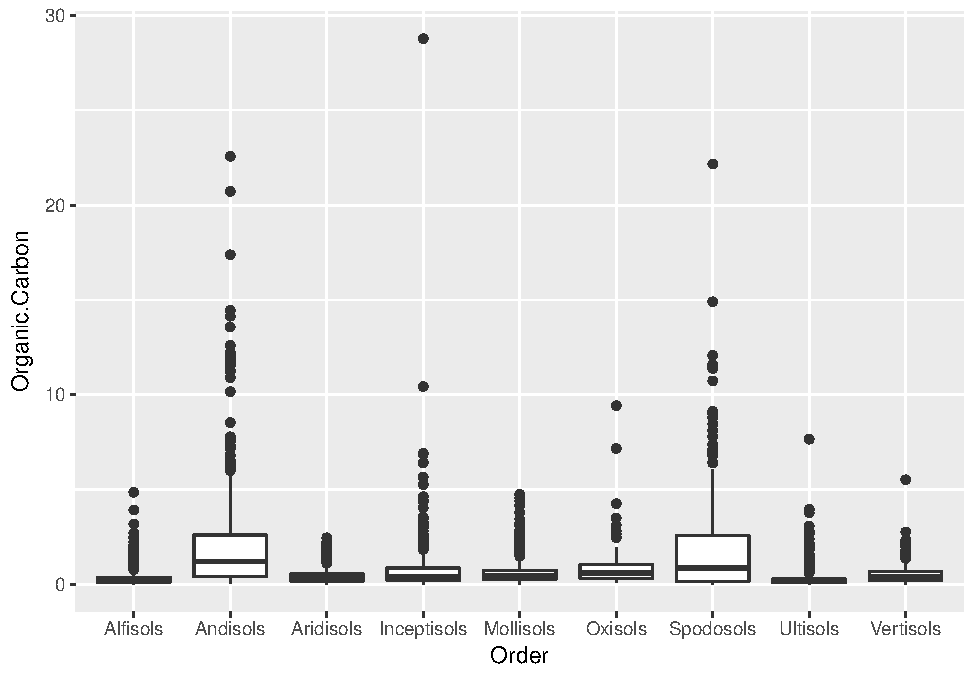
\includegraphics{Project1_files/figure-latex/EDA - Mer-3.pdf}
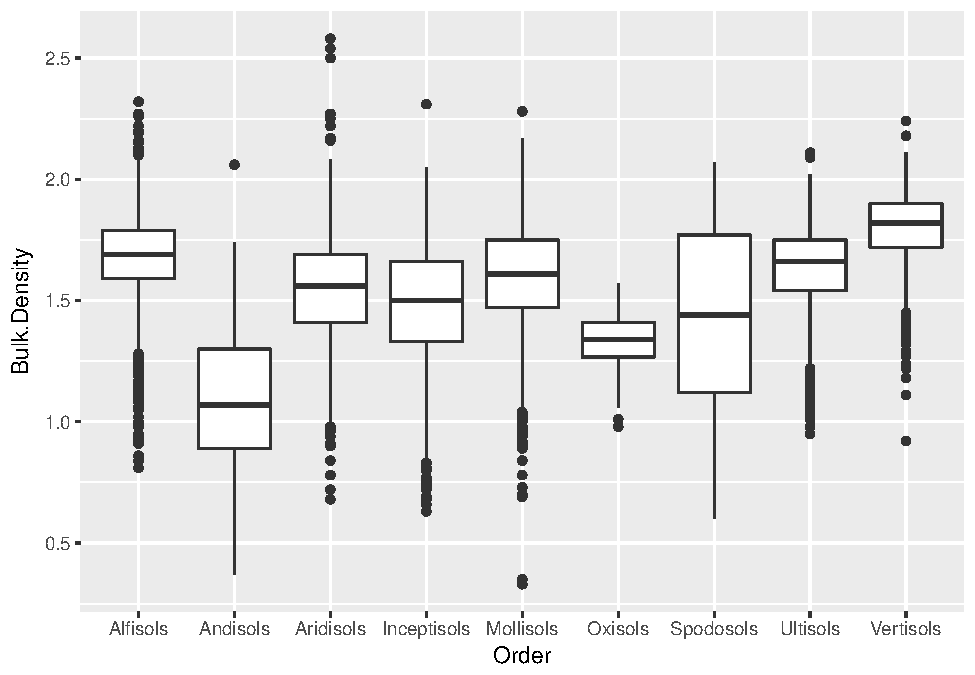
\includegraphics{Project1_files/figure-latex/EDA - Mer-4.pdf}
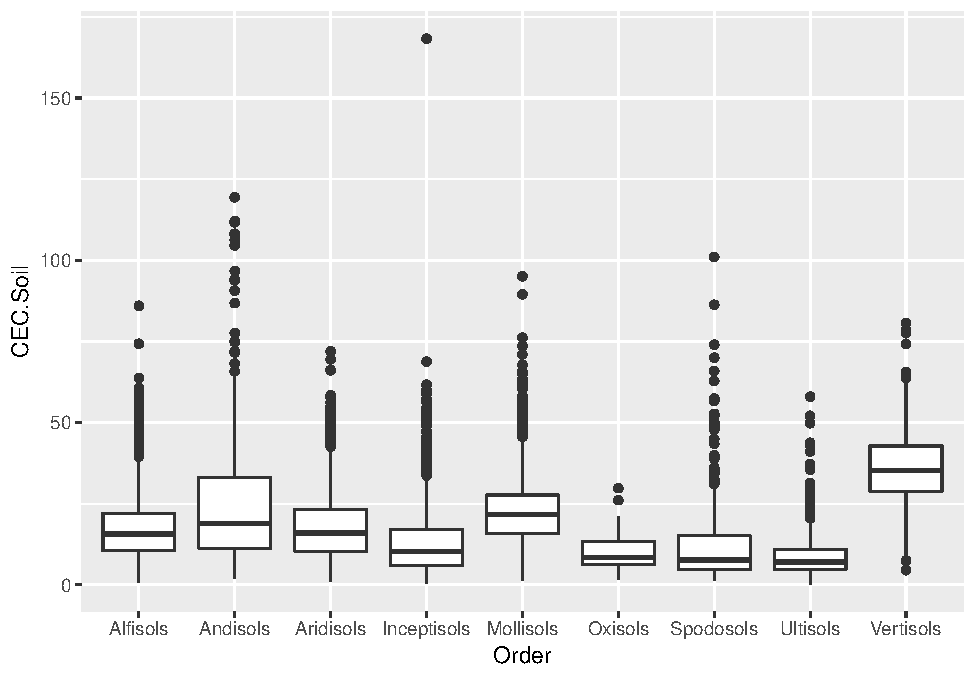
\includegraphics{Project1_files/figure-latex/EDA - Mer-5.pdf}
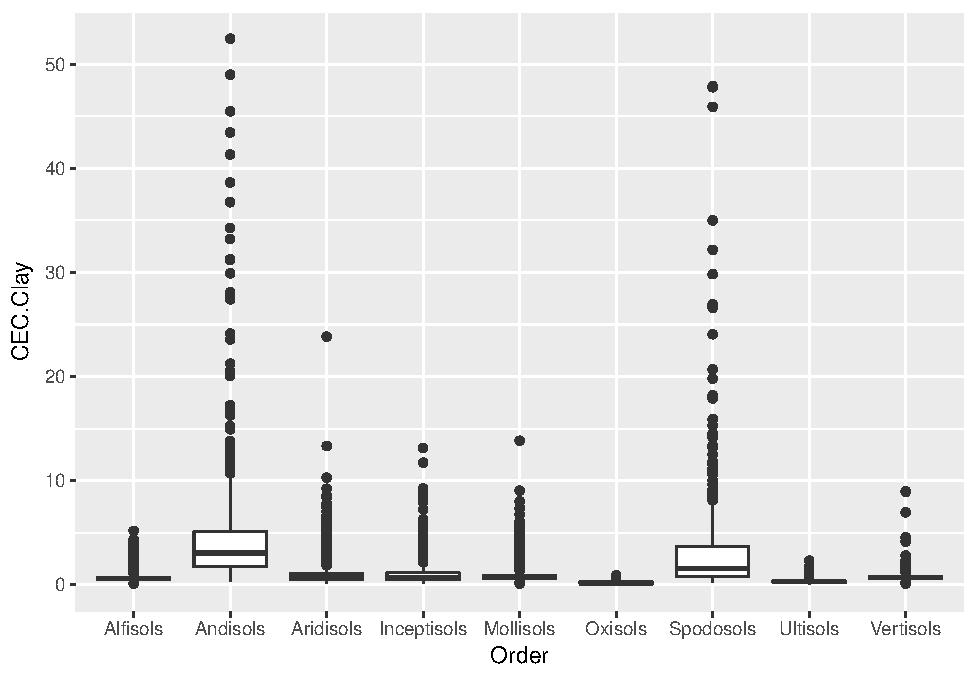
\includegraphics{Project1_files/figure-latex/EDA - Mer-6.pdf}
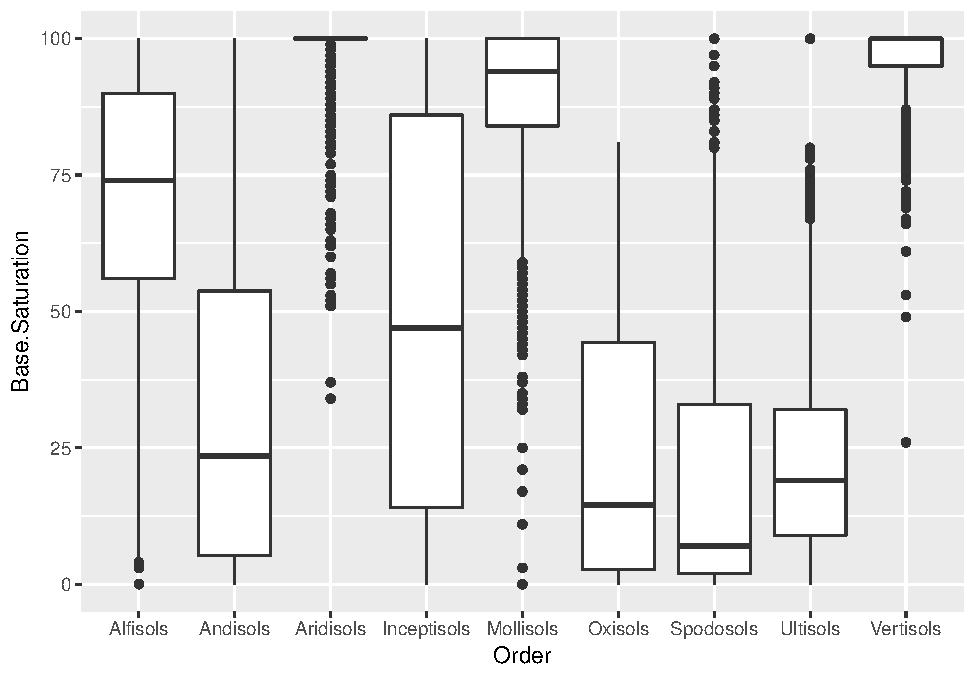
\includegraphics{Project1_files/figure-latex/EDA - Mer-7.pdf}
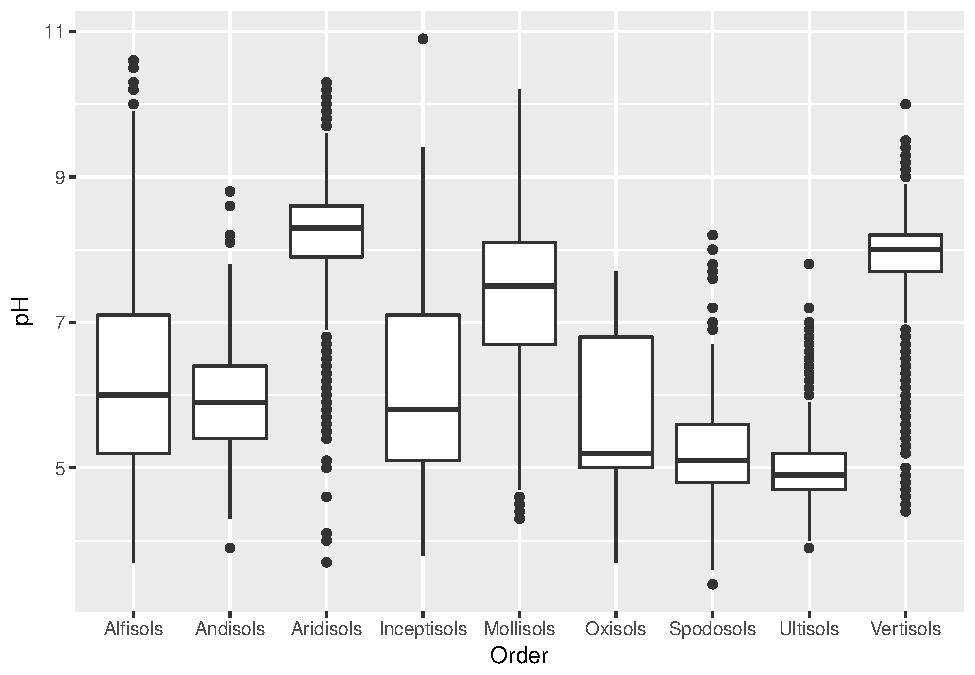
\includegraphics{Project1_files/figure-latex/EDA - Mer-8.pdf}

\section{Analysis}\label{analysis}

\subsection{Linear Discriminant Analysis
(LDA)}\label{linear-discriminant-analysis-lda}

\begin{verbatim}
##    Alfisols    Andisols   Aridisols Inceptisols   Mollisols     Oxisols 
##   0.5756410   0.5135135   0.5312500   0.1226415   0.6719902   0.7058824 
##   Spodosols    Ultisols   Vertisols 
##   0.2674419   0.7413793   0.6056338
\end{verbatim}

\begin{verbatim}
## [1] 0.5676163
\end{verbatim}

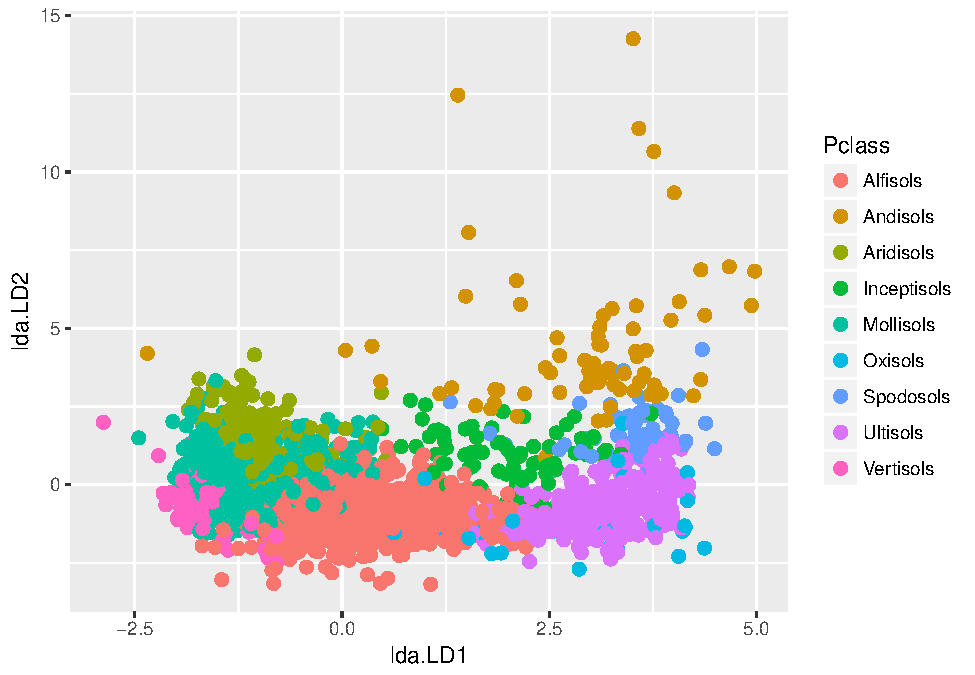
\includegraphics{Project1_files/figure-latex/LDA - Fei-1.pdf}

\subsection{Quadratic Discriminant
Analysis}\label{quadratic-discriminant-analysis}

\begin{verbatim}
##    Alfisols    Andisols   Aridisols Inceptisols   Mollisols     Oxisols 
##   0.7025641   0.3648649   0.5528846   0.1745283   0.5233415   0.8235294 
##   Spodosols    Ultisols   Vertisols 
##   0.3720930   0.8362069   0.6830986
\end{verbatim}

\begin{verbatim}
## [1] 0.5787955
\end{verbatim}

\subsection{Multinomial Logistic
Regression}\label{multinomial-logistic-regression}

\begin{verbatim}
## # weights:  90 (72 variable)
## initial  value 24413.362279 
## iter  10 value 15571.788617
## iter  20 value 15002.934730
## iter  30 value 14478.067709
## iter  40 value 13342.947004
## iter  50 value 12895.100142
## iter  60 value 11964.921219
## iter  70 value 11392.960138
## iter  80 value 11092.884124
## iter  90 value 11073.376567
## iter 100 value 11068.820796
## final  value 11068.820796 
## stopped after 100 iterations
\end{verbatim}

\begin{verbatim}
## Call:
## nnet::multinom(formula = Order ~ ., data = project1data, subset = logr_train)
## 
## Coefficients:
##             (Intercept)         Sand        Clay Organic.Carbon
## Andisols      -1.257580  0.004604636 -0.14837098      1.4814836
## Aridisols    -16.647205  0.037371622  0.01397444      1.8354158
## Inceptisols   -1.546126 -0.001386762 -0.02952812      1.5541408
## Mollisols     -4.784262 -0.010040832 -0.03849970      2.1073975
## Oxisols       -1.228724 -0.036673998  0.12533802      1.5804614
## Spodosols      3.154741 -0.002459725 -0.30013019      2.0265253
## Ultisols       4.176125  0.020686544  0.02329184      0.9611524
## Vertisols    -25.756763 -0.032795642  0.02686232      1.1029453
##             Bulk.Density     CEC.Soil   CEC.Clay Base.Saturation
## Andisols      -3.3268648  0.090699690  0.7283956     -0.05400634
## Aridisols     -2.9977783  0.017788300  0.7767474      0.08904043
## Inceptisols   -1.5721995 -0.033087145  0.6996854     -0.05024397
## Mollisols     -1.1448023  0.047291014  0.5020496      0.04673994
## Oxisols       -5.4297005 -0.384503261 -0.9479182     -0.14023916
## Spodosols      0.8954668  0.002404581  0.7267122     -0.02971002
## Ultisols      -0.5523640 -0.029525291 -6.0788610     -0.07628861
## Vertisols      3.7233981  0.101828103  0.8685522      0.07153714
##                      pH
## Andisols     1.03564767
## Aridisols    1.25567438
## Inceptisols  0.98149835
## Mollisols    0.30925835
## Oxisols      2.07863101
## Spodosols   -0.46243105
## Ultisols     0.06223332
## Vertisols    0.96201601
## 
## Std. Errors:
##             (Intercept)        Sand        Clay Organic.Carbon
## Andisols      1.0310036 0.005048637 0.017763183      0.1323038
## Aridisols     0.7567081 0.002603326 0.006319524      0.1391297
## Inceptisols   0.5795942 0.002545976 0.007085791      0.1273438
## Mollisols     0.4033562 0.001836661 0.005258040      0.1095274
## Oxisols       0.2767875 0.014934380 0.017266353      0.2450583
## Spodosols     1.1548783 0.004945074 0.025558550      0.1459979
## Ultisols      1.0390342 0.003520762 0.010589521      0.1903680
## Vertisols     1.1395826 0.005597663 0.007548138      0.1939263
##             Bulk.Density    CEC.Soil  CEC.Clay Base.Saturation         pH
## Andisols       0.4291549 0.012529912 0.1603186     0.005764099 0.14309326
## Aridisols      0.2374184 0.008514832 0.1549128     0.007760952 0.07389334
## Inceptisols    0.2665768 0.010696741 0.1580458     0.003296969 0.07042780
## Mollisols      0.1922521 0.007539809 0.1536843     0.003460284 0.04776292
## Oxisols        0.7171407 0.065117056 1.2830235     0.013121106 0.24593297
## Spodosols      0.4031730 0.019898739 0.1622694     0.005147604 0.15985335
## Ultisols       0.3992114 0.025454237 0.7309696     0.004329235 0.12335749
## Vertisols      0.3997487 0.009602013 0.1887096     0.012469922 0.10947987
## 
## Residual Deviance: 22137.64 
## AIC: 22281.64
\end{verbatim}

\section{Results}\label{results}

The results from these three approaches show that\ldots{}

In order to compare the reults it is important to recall the diffences
between these three classification approaches. The difference between
LDA and logistic regression is that linear coefficients are estimated
differently. MLE for logistic models and estimated mean and variance
based on Gaussian assumptions for the LDA. LDA makes more restrictive
Gaussian assumptions and therefore often expected to work better than
logistic models IF they are met. QDA serves as a compromise between
non-parametric methods (not explored in this project) and the linear LDA
and logistic regression approaches. Since QDA assumes a quadratic
decision boundary, it can accurately model a wider range of problems
than can the linear methods. QDA can perform better in the presence of a
limited number of training observations because it does make some
assumptions about the form of the decision boundary.

\section{Contributions}\label{contributions}


\end{document}
